\documentclass[]{book}
\usepackage{lmodern}
\usepackage{amssymb,amsmath}
\usepackage{ifxetex,ifluatex}
\usepackage{fixltx2e} % provides \textsubscript
\ifnum 0\ifxetex 1\fi\ifluatex 1\fi=0 % if pdftex
  \usepackage[T1]{fontenc}
  \usepackage[utf8]{inputenc}
\else % if luatex or xelatex
  \ifxetex
    \usepackage{mathspec}
  \else
    \usepackage{fontspec}
  \fi
  \defaultfontfeatures{Ligatures=TeX,Scale=MatchLowercase}
    \setmainfont[]{Open Sans}
\fi
% use upquote if available, for straight quotes in verbatim environments
\IfFileExists{upquote.sty}{\usepackage{upquote}}{}
% use microtype if available
\IfFileExists{microtype.sty}{%
\usepackage{microtype}
\UseMicrotypeSet[protrusion]{basicmath} % disable protrusion for tt fonts
}{}
\usepackage[margin=1in]{geometry}
\usepackage{hyperref}
\hypersetup{unicode=true,
            pdftitle={Атлас Российского пограничья},
            pdfauthor={Лаборатория геополитических исследований ИГ РАН},
            pdfborder={0 0 0},
            breaklinks=true}
\urlstyle{same}  % don't use monospace font for urls
\usepackage{natbib}
\bibliographystyle{apalike}
\usepackage{longtable,booktabs}
\usepackage{graphicx,grffile}
\makeatletter
\def\maxwidth{\ifdim\Gin@nat@width>\linewidth\linewidth\else\Gin@nat@width\fi}
\def\maxheight{\ifdim\Gin@nat@height>\textheight\textheight\else\Gin@nat@height\fi}
\makeatother
% Scale images if necessary, so that they will not overflow the page
% margins by default, and it is still possible to overwrite the defaults
% using explicit options in \includegraphics[width, height, ...]{}
\setkeys{Gin}{width=\maxwidth,height=\maxheight,keepaspectratio}
\IfFileExists{parskip.sty}{%
\usepackage{parskip}
}{% else
\setlength{\parindent}{0pt}
\setlength{\parskip}{6pt plus 2pt minus 1pt}
}
\setlength{\emergencystretch}{3em}  % prevent overfull lines
\providecommand{\tightlist}{%
  \setlength{\itemsep}{0pt}\setlength{\parskip}{0pt}}
\setcounter{secnumdepth}{5}
% Redefines (sub)paragraphs to behave more like sections
\ifx\paragraph\undefined\else
\let\oldparagraph\paragraph
\renewcommand{\paragraph}[1]{\oldparagraph{#1}\mbox{}}
\fi
\ifx\subparagraph\undefined\else
\let\oldsubparagraph\subparagraph
\renewcommand{\subparagraph}[1]{\oldsubparagraph{#1}\mbox{}}
\fi

%%% Use protect on footnotes to avoid problems with footnotes in titles
\let\rmarkdownfootnote\footnote%
\def\footnote{\protect\rmarkdownfootnote}

%%% Change title format to be more compact
\usepackage{titling}

% Create subtitle command for use in maketitle
\newcommand{\subtitle}[1]{
  \posttitle{
    \begin{center}\large#1\end{center}
    }
}

\setlength{\droptitle}{-2em}

  \title{Атлас Российского пограничья}
    \pretitle{\vspace{\droptitle}\centering\huge}
  \posttitle{\par}
    \author{Лаборатория геополитических исследований ИГ РАН}
    \preauthor{\centering\large\emph}
  \postauthor{\par}
      \predate{\centering\large\emph}
  \postdate{\par}
    \date{2018-11-22}

\usepackage{booktabs}
\usepackage{amsthm}
\makeatletter
\def\thm@space@setup{%
  \thm@preskip=8pt plus 2pt minus 4pt
  \thm@postskip=\thm@preskip
}
\makeatother

\begin{document}
\maketitle

{
\setcounter{tocdepth}{1}
\tableofcontents
}
\chapter*{Введение}
\addcontentsline{toc}{chapter}{Введение}

Атлас подготовлен в результате реализации исследовательского проекта
Российского научного фонда «Российское пограничье: вызовы соседства»
(грант №14-18-03621) и представляет собой комплексное научно-справочное
картографическое произведение, призванное дать целостное представление о
развитии приграничных регионов России и сопредельных стран. Атлас носит
междисциплинарный и проспективный характер и допускает постоянное
обновление информации. В его основу положен принцип полимаштабности:
проблемы пограничья показаны на четырех уровнях -- макрорегиональном,
общегосударственном, региональном и локальном. Он объединяет карты,
отражающие ситуацию вдоль всей линии российской границы с обеих ее
сторон в европейской и азиатской частях российского пограничья и на их
детально изученных на муниципальном уровне ключевых участках пограничья.
Использованы передовые способы картографирования границ -- от нанесения
точечной экспертной информации до автоматизированной обработки данных
дистанционного зондирования, пространственного анализа и интерполяции
средствами ГИС.

Атлас охватывает широкий круг проблем в сфере внешних связей, экономики,
социальной и этнокультурной ситуации, охраны окружающей среды в
приграничных регионах России и сопредельных стран. Значительное внимание
уделено влиянию на развитие приграничного сотрудничества режима и
функционирования границы в целом, исторической памяти и массовых
стереотипов, «фантомным границам», утратившим свои главные функции, но
продолжающим влиять на отношения людей и принимаемые решения. Интегрируя
разнообразную информацию в разрезе всего пограничья и его отдельных
частей, атлас представляет ее в систематизированной, сопоставимой и
хорошо обозримой форме.

Атлас содержит, во-первых, карты на традиционные сюжеты (дифференциации
пограничья по демографическим и социально-экономическим показателям,
морфологии российских границ по «возрасту» и происхождению,
легитимности, этнической контрастности, экологических взаимосвязей и
трансграничных угроз); во-вторых, карты на новые, неизвестные ранее темы
(потенциал трансграничного сотрудничества, объекты нового строительства,
роль границ в этнических и иных конфликтах, барьерность границ,
повседневная жизнь и мотивы приграничной мобильности населения,
историко-символический ландшафт, фантомные границы); в-третьих, карты на
основе инновационных методов картографирования (плотности автодорожной
сети, населенных пунктов, динамики землепользования и лесопользования).

В работе восемь разделов: «Геополитическое положение», «Население»,
«Уровень жизни населения», «Экономика», «Динамика трансграничных
взаимодействий», «Развитие трансграничных систем и экологические
угрозы», «Конфликты в приграничье», «Соотношение культурных, ментальных
и институциональных границ». Атлас содержит 85 карт в разном масштабе,
их аналитические описания, табличный, графический и другой
дополнительный материал и ориентирован на специалистов в области
международных отношений и приграничного сотрудничества, а также на
широкий круг читателей, интересующихся изучением российского пограничья
(пограничными исследованиями).

\chapter{Население}\label{pop}

\section{Размещение и плотность населения}\label{demo-dens}

Приграничные регионы России -- это 27\% территории страны (4,6 млн. кв.
км.), где проживает 67 млн. чел. или немногим менее половины российского
населения (45,6\%). Общая площадь приграничных регионов соседних стран
составляет 5,9 млн. кв. км., а их население -- около 148 млн. чел.,
примерно вдвое больше, чем с российской стороны границы. Однако, если
рассматривать полосу муниципальных районов, расположенных в
непосредственной близости от границы, то ситуация заметно варьирует.
Градиенты плотности населения и различия в его размещении в значительной
мере определяются природными (горы, реки, озера и пр.), историческими
(события прошлого и особенности освоения территории) и геополитическими
факторами. Так, следствием дезинтеграции СССР и образования новых
постсоветских государств стало формирование новой пограничной зоны.
Сегодня здесь проживает свыше 90\% жителей всего российского
приграничья.

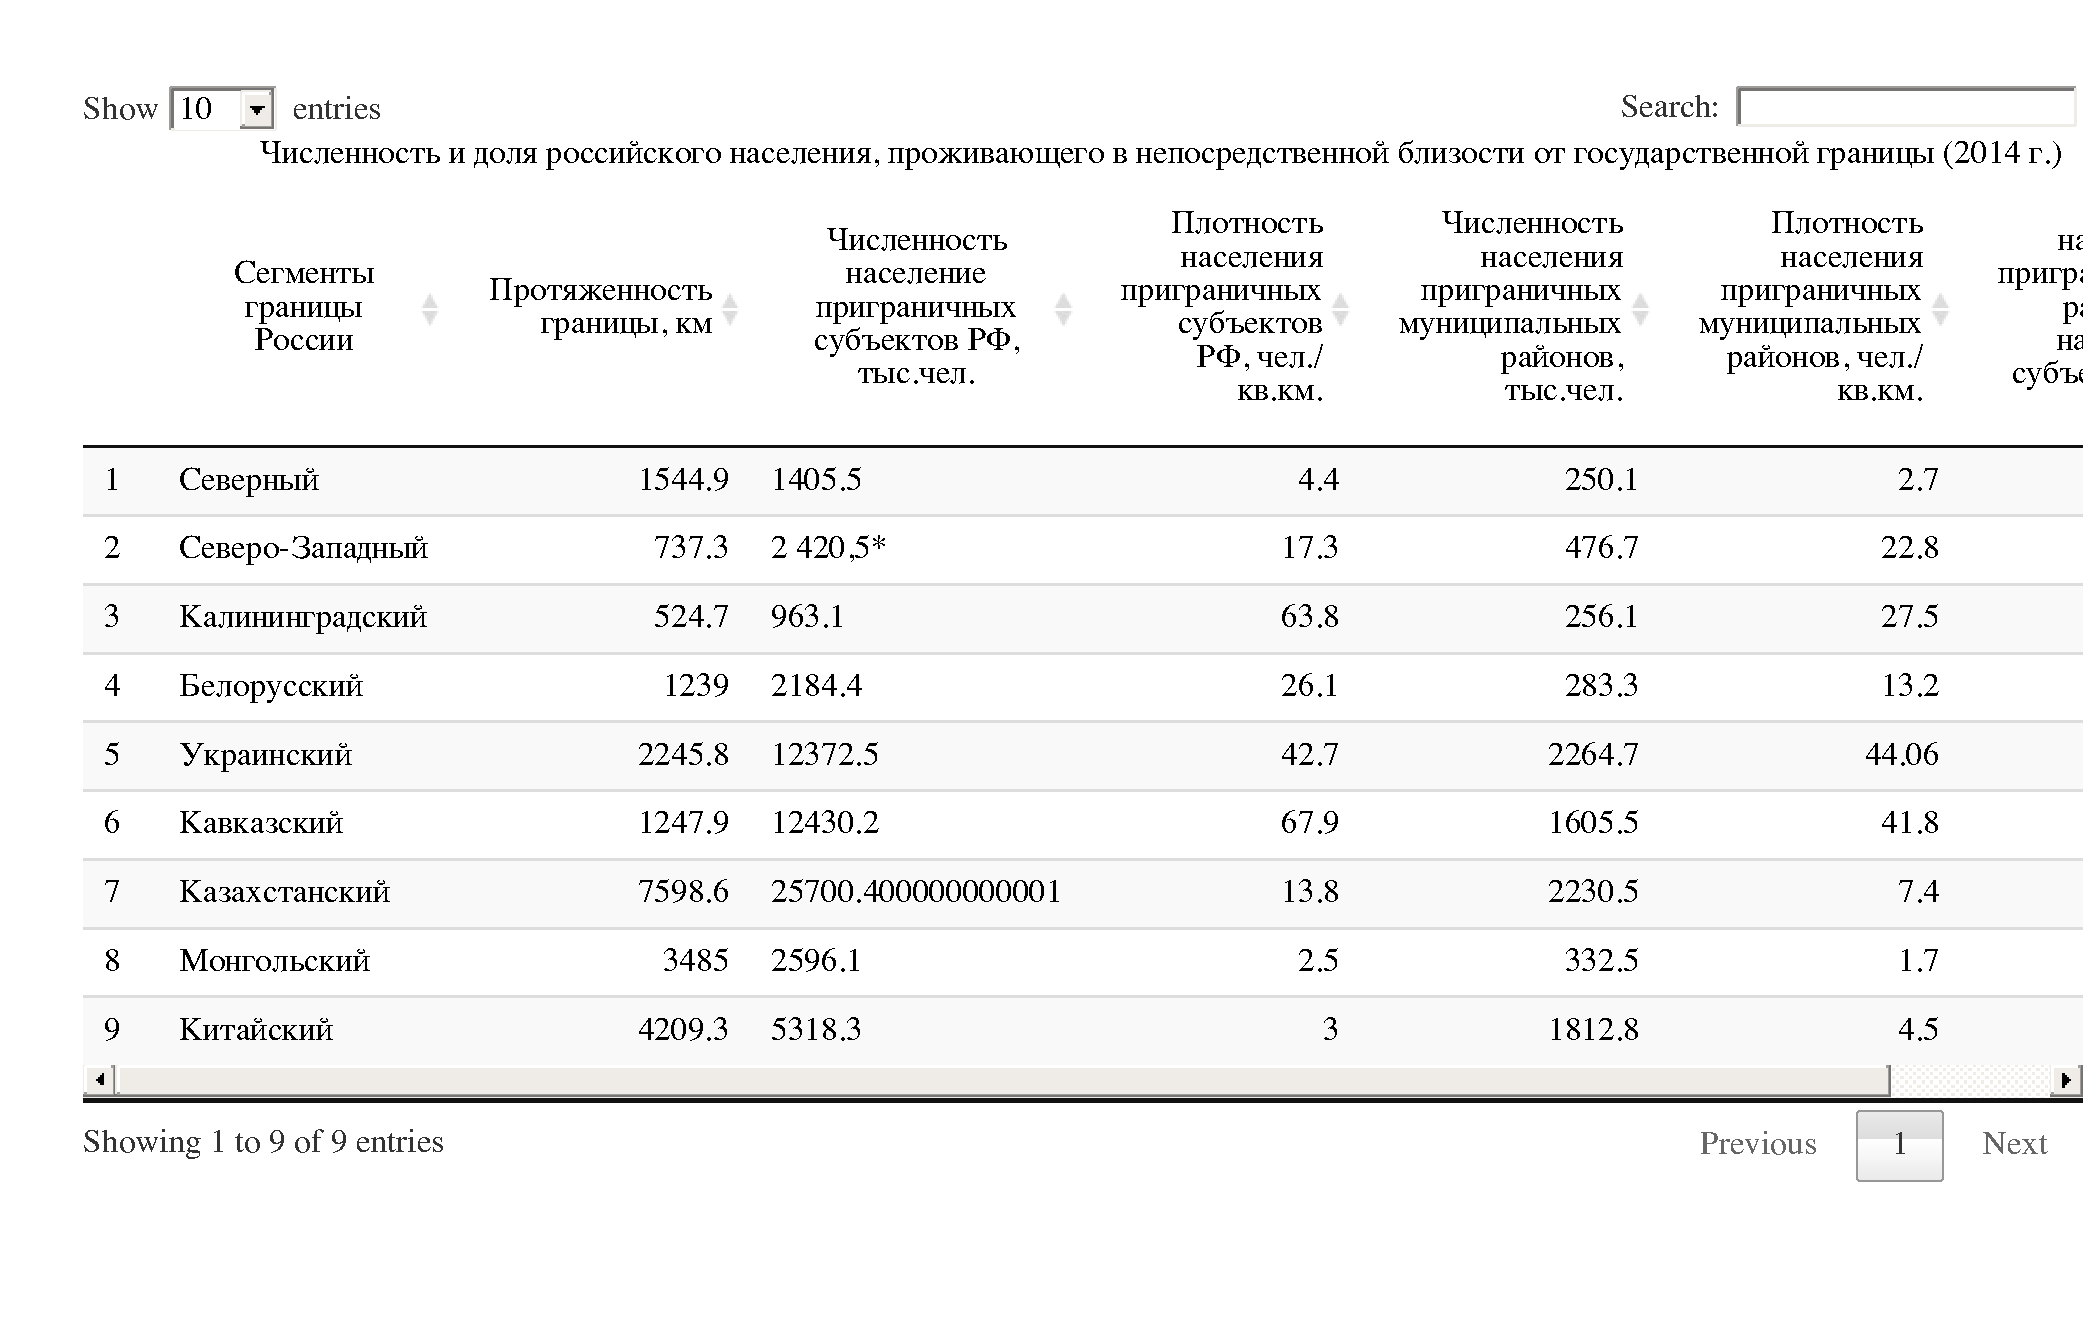
\includegraphics{02-Demography_files/figure-latex/unnamed-chunk-1-1.pdf}

«Маршрут» линии российской границы наглядно проявляет различия в ее
морфологии, происхождении и размещении населения. Если граница РФ с
Норвегией и Балтийскими странами в значительной мере проходит по водным
рубежам (рекам и озерам), а в Финляндии она разделяет относительно
слабозаселенные районы восточной и западной Карелии, то на участке от
Балтийского до Азовского морей -- зону высокой плотности населения и
интенсивного хозяйственного освоения. В целом, на западном и
юго-западном отрезках границы градиенты плотности населения сложились не
в пользу РФ. За немногими исключениями приграничные районы сопредельных
стран имеют более высокую плотность населения и уровень хозяйственного
освоения. Даже Ленинградская область практически в два раза отстает от
старопромышленного региона Ида-Вирумаа в Эстонии. На Кавказе граница
вновь возвращается к природным рубежам. Здесь, несмотря на высокую
численность населения, приграничные горные районы являются
труднодоступными и малонаселенными. Дальше на восток линия границы
проходит южнее основной полосы расселения бывшего СССР, пересекая степи
Заволжья, Южного Урала и юга Сибири. На этом сегменте границы, напротив,
более заселенными и экономически развитыми являются приграничные районы
РФ, а не Казахстана, относящиеся к зоне очагового расселения. На
монгольском и китайском отрезках границы она вновь возвращается к
природным разграничительным линиям -- горным хребтам Монголии и Южной
Сибири, рекам Амуру, Уссури и Аргунь. Если на границе с Монголией
контрасты в плотности населения практически отсутствуют, по обе стороны
государственной границы она не превышает 3 чел. на кв. км., то на
российско-китайской границе ситуация иная. Даже не слишком заселенная по
китайским меркам провинция Хэйлунцзян превосходит по плотности населения
Приморский край -- наиболее освоенный регион российского Дальнего
востока, в 7,5 раз, а Амурскую область более чем в 40 раз. Однако
демографическое давление Китая на российское пограничье не столь
значительно, как может показаться на первый взгляд. Полоса территорий
китайского пограничья, так же, как и с российской стороны, отличается
очаговостью расселения и значительными малолюдными пространствами. К
тому же для северо-востока Китая характерен миграционный отток населения
в климатически более благоприятные и экономически более развитые
прибрежные регионы юга и юго-востока страны.

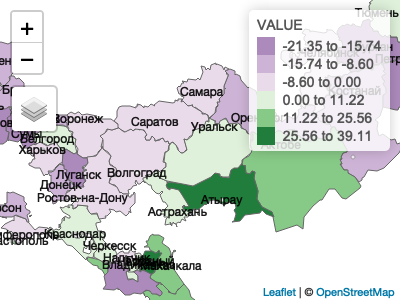
\includegraphics[width=1\linewidth]{02-Demography_files/figure-latex/unnamed-chunk-2-1}

\begin{quote}
Динамика численности населения (2000-2016 гг.)
\end{quote}

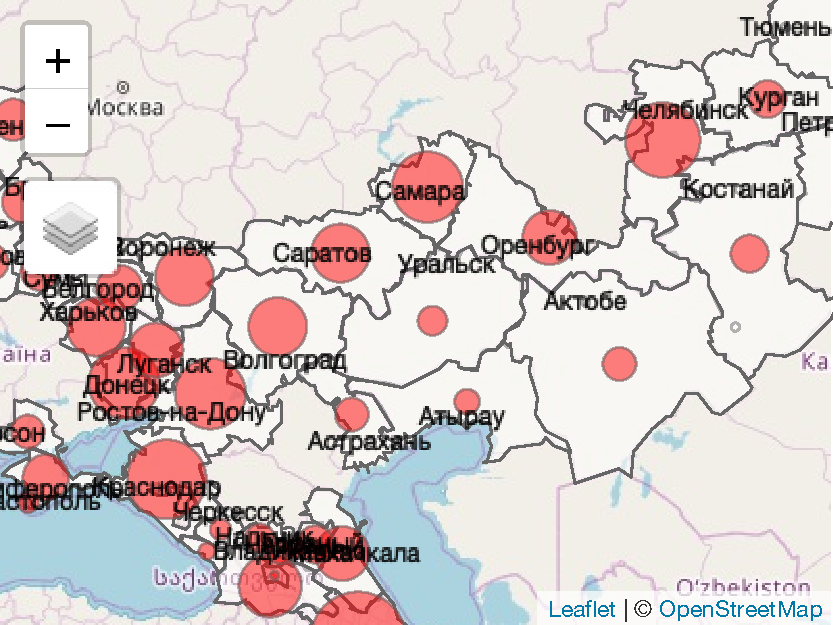
\includegraphics[width=1\linewidth]{02-Demography_files/figure-latex/unnamed-chunk-3-1}

\begin{quote}
Численность населения (2016 г.)
\end{quote}

\section{Городское и сельское расселение}\label{demo-urban}

Российское пограничье в целом более урбанизировано, чем приграничные
территории соседних стран. Непосредственно на границе РФ (в
пятикилометровой пограничной зоне) располагается 17 городов, большинство
-- малые и средние, но есть и крупнейшие, такие как Сочи, агломерация
Орск-Новотроицк и Благовещенск. Список городов, попадающих в
50-километровую приграничную зону, намного длиннее и включает Хабаровск,
Калининград, Псков, Смоленск, Белгород и Астрахань. Для всего периметра
«новых» российских границ характерно наличие тесно связанных между собой
систем расселения, которые сформировались в Северо-Западных и
Центральных регионах бывшего СССР, а также средне урбанизированных
областях Центрального Черноземья и Европейского Юга. В
российско-белорусском и российско-украинском пограничье выделяются пары
или группы городов и населенных пунктов, расположенных вблизи границы и
связанных автомобильными и железными дорогами (например, Себеж --
Верхнедвинск, Шебекино -- Волчанск, Чертково-Меловое, Донецк-Должанск,
Джанкой-Гениченск, и пр.). На российско-украинском сегменте границы
расположены две крупнейшие полицентричные системы расселения: биполярная
Харьковско-Белгородская агломерация, расстояние между центрами которой
составляет менее 70 км., а совокупное население около 3 млн. человек, и
Донецко-Азовская конурбация, охватывающая более 10 млн. человек и
включающая в себя такие крупнейшие города как Донецк, Луганск и
Ростов-на-Дону.

Российско-украинское пограничье -- это также пример относительно
равномерного распределения сельского населения, плотность которого
колеблется в пределах 10-20 чел. на кв. км., и больших различий по обе
стороны границы не наблюдается.

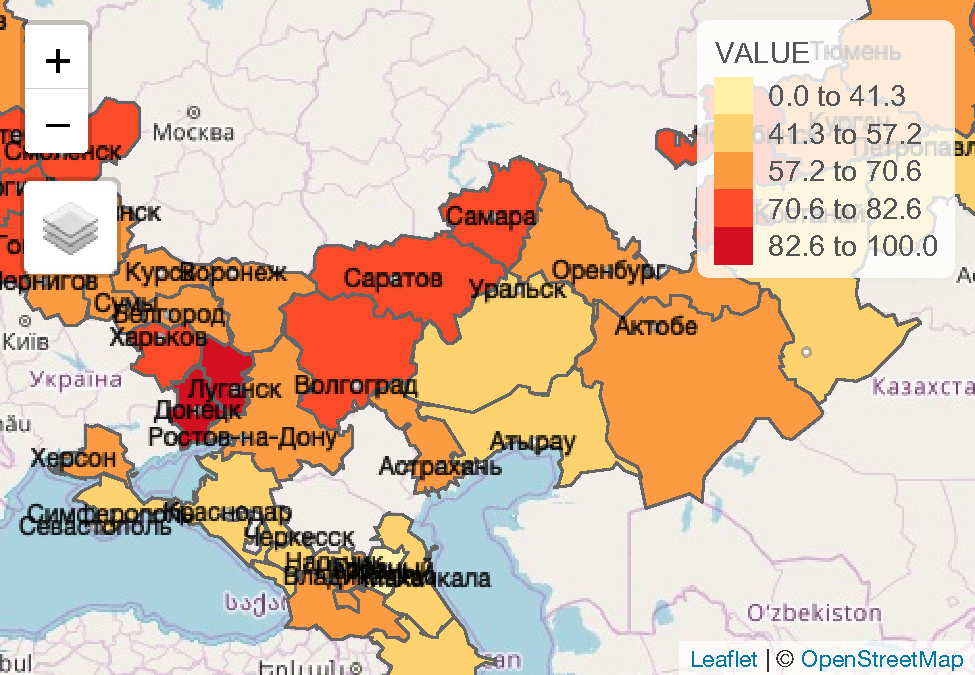
\includegraphics{02-Demography_files/figure-latex/unnamed-chunk-4-1.pdf}

\begin{quote}
Доля городского населения, 2016 г.
\end{quote}

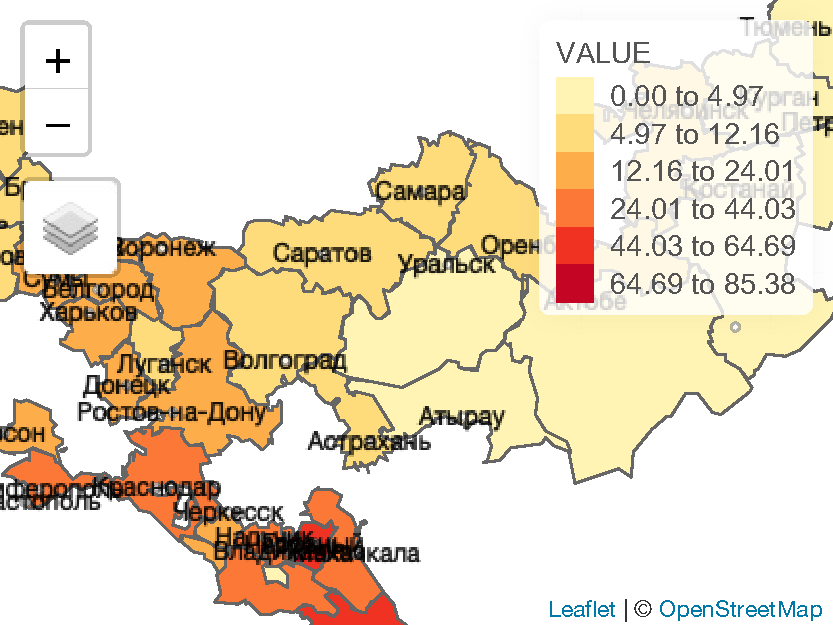
\includegraphics{02-Demography_files/figure-latex/unnamed-chunk-5-1.pdf}

\begin{quote}
Плотность сельского населения, 2016 г.
\end{quote}

Российско-казахстанская граница, напротив, характеризуется значительными
контрастами урбанизированности территорий. В российских приграничных
регионах располагается шесть крупнейших агломераций: Самаро-Тольятинская
(свыше 2,3 млн. чел.), Новосибирская (1,9 млн. чел.), Челябинская (1,5
млн. чел.), Волгоградская (1,4 млн. чел.), Омская (1,2 млн. чел.) и
Саратовская (1,2 млн. чел.), которые исторически оказывали влияние на
развитие соседних регионов Казахстана и продолжают его оказывать
сегодня. Контрастная картина характеризует и размещение сельского
населения. Различия особенно заметны в западной части пограничья, где
даже малонаселенные российские регионы опережают казахстанские
практически в два раза. Наименьшая плотность сельского населения
наблюдается в Актюбинской области (1,03 чел. на кв. км.). Градиент
плотности сельского населения постепенно уменьшается при движении на
восток, в силу снижения численности сельского населения и его плотности
с российской стороны и роста -- с казахстанской. Если в Самарской
области данный социальный индикатор в 14 раз выше, чем в
Западно-Казахстанской, то между Алтайским краем Восточно-Казахстанской
областью наблюдается лишь двукратное превышение. На «старых» границах,
где пограничные системы расселения формировались изолировано, регулярные
трансграничные контакты возникли с распадом СССР. Исключением можно
считать российско-финляндскую границу, которая в современном виде была
оформлена в 1947 году. Наиболее впечатляющие изменения произошли в
российско-китайском пограничье, где стремительно выросли торговые
города, такие как Хэйхэ, Суйфэньхэ, Маньчжурия и др.

\section{Размещение и плотность населения}\label{demo-dens}

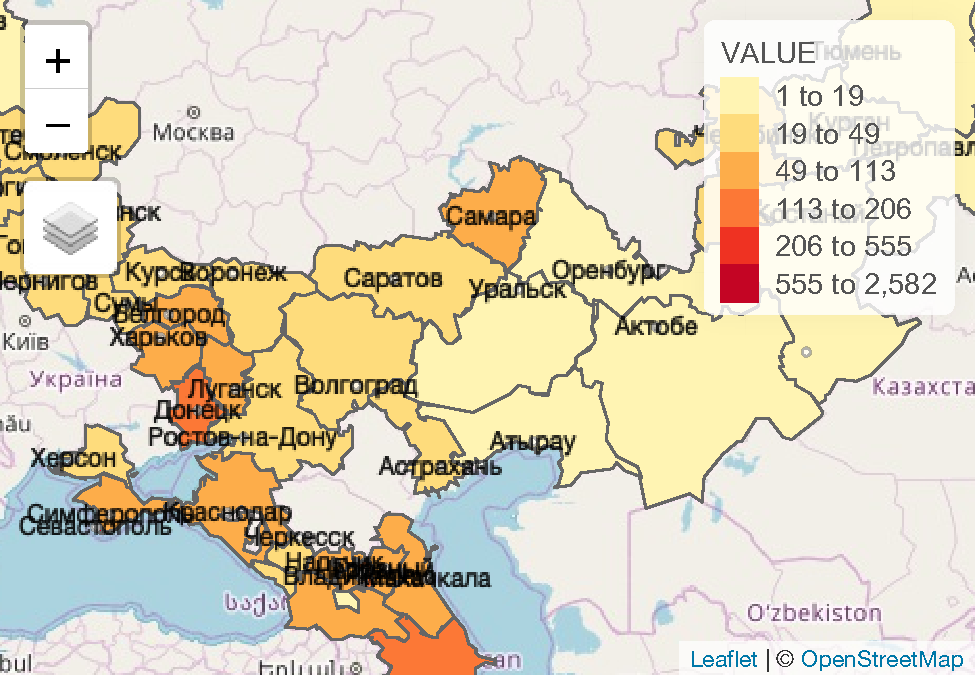
\includegraphics{02-Demography_files/figure-latex/unnamed-chunk-6-1.pdf}

\begin{quote}
Плотность населения, 2016 г.
\end{quote}

\begin{quote}
Плотность населения, 2013 г. (Китай)
\end{quote}

\section{Демографическая ситуация}\label{demo-situ}

\subsection{Численность населения}\label{demo-situ-pop}

Приграничная полоса регионов России в целом характеризуется относительно
стабильной демографической ситуацией с тенденцией к сокращению населения
в результате его естественной убыли и миграционного оттока. За период
2000-2014 годов, статистика зафиксировала сокращение численности
населения в приграничье на 2,4\%, однако этот показатель вряд ли
фиксирует реальное трансграничное миграционное движение и наличие
значительного числа незарегистрированных трудовых мигрантов и
переселенцев. Статистика также показывает высокую вариативность
процессов роста/убыли населения, как в пределах отдельных сегментов
границы, так и регионов, их зависимость от конкретных обстоятельств,
оценок населением выгод и издержек приграничного положения.

\begin{quote}
На северо-западных и западных сегментах российской границы
регистрировались преимущественно показатели убыли населения.
Максимальные значения: убыль составила свыше 10\%, -- отмечались в
Мурманской, Псковской, Смоленской, Брянской и Курской областях, а также
республики Карелия. Похожая ситуация наблюдалась в Восточной Сибири и на
Дальнем Востоке (Забайкальский, Хабаровский и Приморский края, Амурская
область и Еврейская АО).
\end{quote}

Противоположная тенденция наблюдалась на кавказском сегменте границы,
здесь во всех регионах фиксировался рост численности населения -- от
5,5\% в Краснодарском крае до 36,8\% в Дагестане и 78,9\% в Чеченской
Республике. Помимо Северного Кавказ, рост населения отмечался в: 1)
экономически привлекательных для трудовых мигрантов
экспортно-ориентированных регионах РФ: Тюменская, Челябинская и
Белгородская области, 2) крупнейших агломерациях: Ленинградская и
Новосибирская области, и 3) национальных республиках востока страны:
республики Тыва, Алтай и Бурятия. В последнем случае, ключевую роль
играли не миграции, а высокий естественный прирост населения.

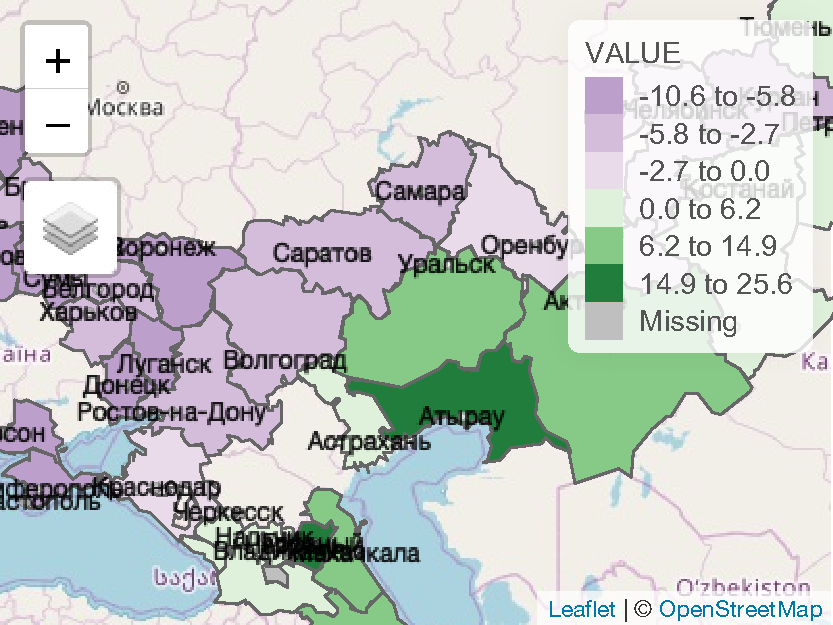
\includegraphics[width=1\linewidth]{02-Demography_files/figure-latex/unnamed-chunk-7-1}

\begin{quote}
Общий коэффициент естественного прироста, 2009 г.
\end{quote}

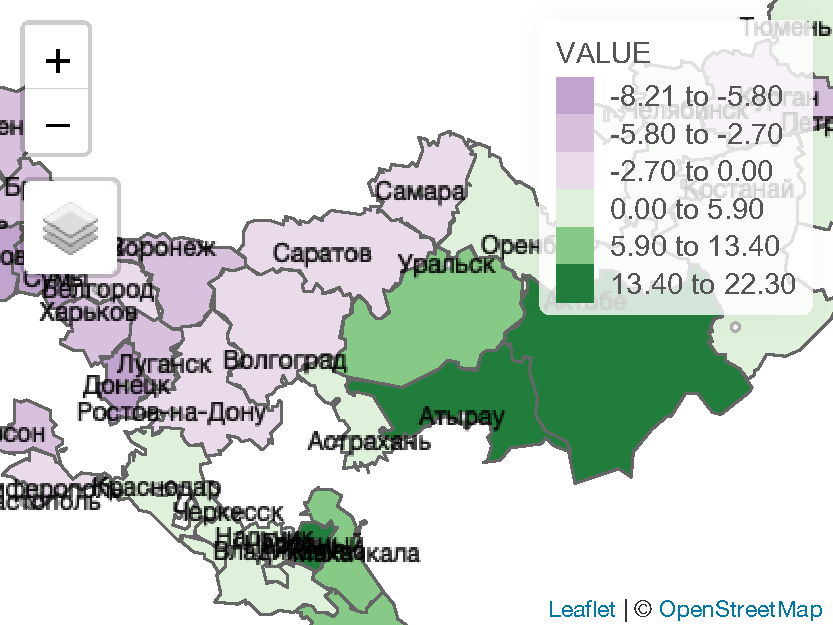
\includegraphics[width=1\linewidth]{02-Demography_files/figure-latex/unnamed-chunk-8-1}

\begin{quote}
Общий коэффициент естественного прироста, 2016 г.
\end{quote}

\begin{quote}
Изменения общего коэффициента рождаемости (ГРАФИК), 2009-2016 гг.
\end{quote}

\begin{quote}
Изменения общего коэффициента смертности (ГРАФИК), 2009-2016 гг.
\end{quote}

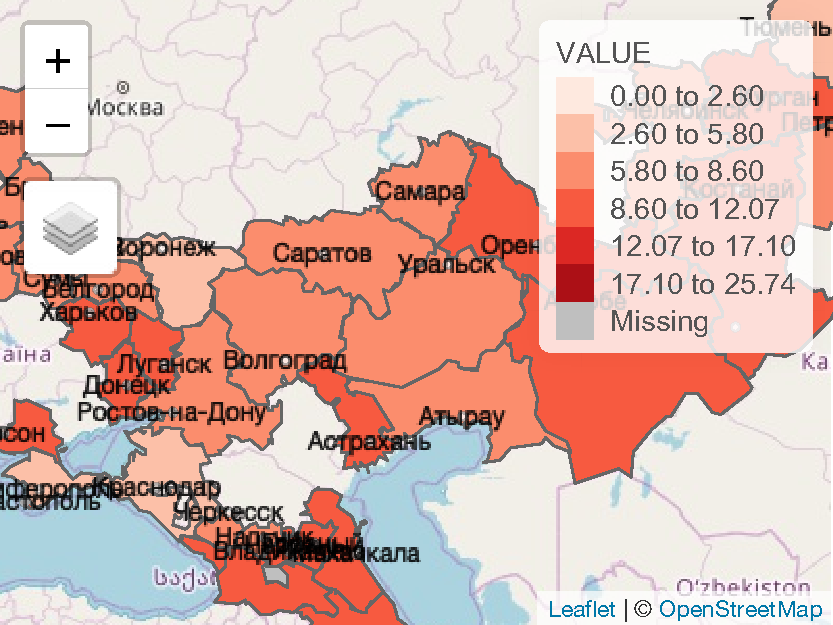
\includegraphics[width=1\linewidth]{02-Demography_files/figure-latex/unnamed-chunk-9-1}
\textgreater{} Общий коэффициент младенческой смертности, 2016 г.

\begin{quote}
ГРАФИК: Изменения общего коэффициента младенческой смертности, 2009-2016
гг.
\end{quote}

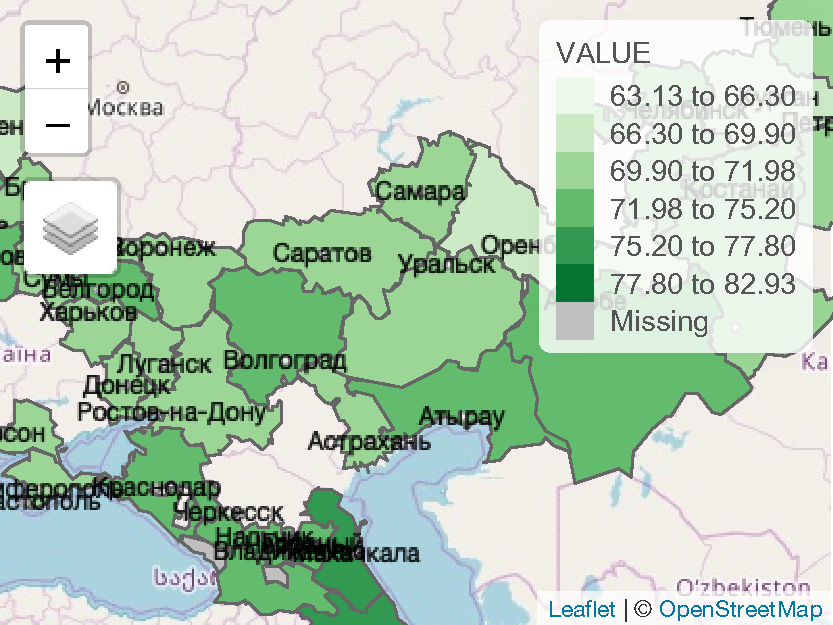
\includegraphics[width=1\linewidth]{02-Demography_files/figure-latex/unnamed-chunk-10-1}
\textgreater{} Ожидаемая продолжительность жизни, 2016 г.

\begin{quote}
Динамика численности населения приграничных субъектов РФ, 2000 - 2012
гг. (\%)
\end{quote}

За тот же период времени население приграничных регионов сопредельных
государств выросло на 1,5\% до 144,1 млн. чел.: 80\% этого прироста
пришлось на приграничные провинции Китая и Монголии, где депопулирующие
российские регионы Сибири (Забайкальский край) и Дальнего Востока
граничат с монгольскими аймаками и китайскими провинциями, традиционно
отличающимися стабильными темпами роста населения. Значительны также
различия в динамике населения между регионами Поволжья (Волгоградская,
Самарская, Саратовская, Оренбургская области) и нефтегазовыми регионами
Западного Казахстана (Атырауская, Западно-Казахстанская, Актюбинская
области), где отмечается заметный рост населения. Сказалась также
целенаправленная политика правительства Казахстана по переселению на
север и северо-восток страны как оралманов (казахов-репатриантов), так и
жителей трудоизбыточных южных регионов страны.

Для западных соседей России были характерны скорее процессы убыли
населения. Так, в Латгалии (Восточная Латвия) население сокращалось
вдвое быстрее, чем в среднем по Латвии. Аналогичная картина в
Белоруссии, где население трех пограничных с Россией областей Белоруссии
уменьшилось за 2000--2014 годы на 10\% при среднем для страны показателе
убыли населения 5,3\%, и на Украине, где названное соотношение
составляют 12,5\% и 7,9\%. Эти процессы связаны не только с
демографическим кризисом, переживаемым всеми постсоветскими странами, но
и экономической периферизацией приграничных районов.

\subsection{Естественное движение населения}\label{demo-situ-re}

В последнее десятилетие естественное воспроизводство населения в России
характеризуется незначительным ростом рождаемости и медленным снижением
смертности. Этим тенденциям соответствует и ситуация в российском
пограничье. Тем не менее, ситуация остается достаточно критической
практически во всем приграничье. Если в 2009 году естественный прирост
населения наблюдался только в 12 регионах -- южных и сибирских
национальных республиках, в Тюменской и Астраханской областях, то в 2014
году к этому списку добавились Новосибирская, Челябинская, Омская,
Оренбургская, Сахалинская, Мурманская области, Краснодарский,
Ставропольский и Хабаровский край. Ключевую роль в обеспечении
положительных тенденций естественного воспроизводства населения играют
его более «молодой» возрастной состав и этнические различия в
демографическом поведении русских и других народов страны.

В сопредельных странах ситуация частично похожа на российскую, а
частично -- отличается. Отрицательные показатели естественного движения
населения характеризуют украинский, белорусский и прибалтийский сегменты
границы и слабо положительные -- норвежский, финляндский и частично
польский. На Кавказе, напротив, отмечается естественный прирост
населения на фоне его миграционной убыли. В Грузии отток населения из
приграничья, вызванный как экономическими причинами, так и острыми
территориальными конфликтами в грузино-российском пограничье, привели к
2014 году к ухудшению демографической ситуации и смене тренда
естественного прироста населения на его убыль. Далее при движении на
восток в приграничных регионах сопредельных стран наблюдается
положительная динамика процесса естественного воспроизводства населения.

\subsection{Рождаемость}\label{demo-situ-bir}

На протяжении всего европейского сегмента российской границы фиксируются
невысокие значения общего показатели рождаемости (9-12‰), различия между
соседними странами -- минимальны. Высокой рождаемостью характеризуются
национальные республики РФ -- Чечня, Ингушетия, Дагестан, Тыва, Алтай и
Бурятия (18-29‰), а также сопредельные районы Азербайджана и аймаки
Монголии. Невысокая рождаемость отличает и соседние с Россией провинции
Китая вследствие проводимой этой страной демографической политики. Не
высоки градиенты и на дальневосточных границах из-за ограничения
рождаемости в Китае. Таким образом, существенные различия в показателях
рождаемости отличают только российско-казахстанский сегмент границы,
особенно на участке между Западно-Казахстанской областью и регионами
Поволжья.

На протяжении последних пяти лет ситуация с рождаемостью несколько
улучшалась во всех приграничных регионах РФ, и скорее ухудшалась или
оставалась без изменений в приграничье сопредельных стран. Тенденции к
снижению рождаемости отмечались в Финляндии Эстонии, Польше, Украине,
Грузии, Китае и Монголии.

\subsection{Смертность}\label{demo-situ-dea}

Демографическое неблагополучие приграничных российских регионов связано
в основном с сохраняющемся высоким уровнем смертности населения,
превышающим среднероссийский показатель (13‰). Максимальные значения
общих коэффициентов смертности зафиксированы в сильно «постаревших»
приграничных областях Европейской России: Псковской, Смоленской,
Брянской, Воронежской и Ленинградской (17-21‰).

Высокая смертность наблюдается и в соседних приграничных регионах
Беларуси и Украины (16-19 ‰), а также стран Балтии (14-15‰). Градиенты
показателей смертности более заметны на границе с Монголией и Китаем,
где благодаря высокой доле молодого населения показатели смертности
низкие. Другие причины -- состояние системы здравоохранения и образ
жизни населения -- обуславливают лучшую ситуацию со смертностью в
приграничных районах Польши, Норвегии и Финляндии. Обратный градиент
характерен для Кавказа, где российские республики с невысокими
показателями смертности населения благодаря высокой доле молодежи
соседствуют с краями Грузии, где показатели смертности заметно выросли.

За последнее пятилетие отмечается положительная динамика показателей
общей смертности и ее структуры. В первую очередь это заметно в Карелии
и Ленинградской области, где сократились различия с соседними регионами
стран ЕС (Финляндией, Эстонией, Литвой, Польшей). Напротив, градиенты
выросли на границе с Беларусью и Западным Казахстаном, где к 2014 году
общие коэффициенты смертности сократились сильнее, чем в соседних
российских регионах.

\subsection{Младенческая смертность}\label{demo-situ-bab}

Младенческая смертность -- один из важнейших индикаторов
социально-экономического развития страны и благополучия ее населения.
Несмотря на наблюдающееся улучшение ситуации в приграничных регионах,
она все еще выглядит хуже общероссийской (k младенческой смертности =
7,4‰). Уровень младенческой смертности во многом определяется
возможностями выявления и профилактики патологий беременности и
выхаживания новорожденных, условиями жизни ребенка в семье после
рождения. Наиболее тревожные показатели младенческой смертности имеют
республики Северного Кавказа, (Ингушетия, Чечня и др.), а также Сибири и
Дальнего Востока (Тыва, Еврейская автономная область и др. Так, в
большинстве приграничных районов Монголии младенческая смертность выше
рекордных для России показателей Республики Тыва (15‰) в 1,5-2,5 раза.
Ситуация обратная на западном периметре границ, где у российских соседей
уровень жизни несколько выше, а уровень младенческой смертности -- ниже.
Особенно эти отличия заметны на границе со странами Северной Европы, где
показатели младенческой смертностью существенно ниже, даже чем в среднем
для стран Евросоюза (3‰). Единственным исключением является
российско-украинское пограничье.

\subsection{Продолжительность жизни}\label{demo-situ-long}

Ожидаемая продолжительность жизни при рождении -- это один из наиболее
часто используемых интегральных показателей, позволяющих оценить
социально-демографические тенденции, характерные для страны. За
последние годы по всему периметру российских границ был зафиксирован
рост продолжительности жизни в среднем на два года. В 20 регионах этот
показатель имеет значения близкие к общероссийским (70,8 лет), однако в
некоторых регионах европейской части страны (Псковская, Смоленская и
Брянская области) и большинстве -- Сибири и Дальнего Востока этот
показатель ниже. На Дальнем Востоке он не превышает 67 лет, а в
республике Тыва -- 62 года. Долгожительством традиционно отличаются
регионы Северного Кавказа (Ингушетия -- 79 лет, Дагестан -- 75,6 лет).
Несмотря на демонстрируемую положительную динамику, российское
пограничье все еще существенно отстает от своих соседей в европейской
части страны. Продолжительность жизни в Норвегии составляет 82 года,
Финляндии -- 81 год, в странах Балтии: Литве -- 74 года, Эстонии -- 77
лет. Обгоняет РФ и Белоруссия -- 73 года.

Следует отметить, что показатель ожидаемой продолжительности жизни не
позволяет адекватно оценить социально-демографическую ситуацию,
во-первых, из-за миграционных перетоков населения, и во-вторых, из-за
недостаточной достоверности данных, отсутствия информации о возрастной
структуре смертности и ее годовых режимах, а также различий в системах
учета. Например, в Китае информация раскрывается далеко не полностью, а
в Монголии существует выраженный недоучет смертности в отдаленных и
малодоступных приграничных районах.

\subsection{Миграции}\label{demo-situ-mig}

Миграции -- это один из наиболее серьезных вызовов развитию приграничных
регионов, испытывающих как миграционный отток «своего» населения в
другие регионы страны и за рубеж, так и его замещение, благодаря притоку
трудовых мигрантов и переселенцев из ближайших регионов соседних стран.
Наиболее серьезной проблемой для пограничья стал «негативный отбор»
населения, сказывающийся на качестве трудовых ресурсов и населения в
целом. Диспропорции российского рынка труда привели к тому, что только
13 приграничных регионов получают молодое трудоспособное население, а
остальные его теряют. Миграционный отток населения достиг своих
максимальных значений в Мурманской и Сахалинской областях, Еврейской АО,
Тыве и Забайкальском крае. Тюменская, Новосибирская, Ленинградская,
Калининградская, Белгородская области и Краснодарский край, напротив,
характеризуются значительным миграционными притоком населения, сдвигами
в его возрастном и этническом составе. В трех приграничных регионах:
Белгородской, Ленинградской и Калининградской областях -- миграционный
прирост полностью компенсирует естественную убыль населения, обеспечивая
положительную динамику его численности.

В регионах соседних стран миграционный отток населения был еще более
заметен. Наиболее тяжелая ситуация сложилась в странах Балтии, где
открытие европейского рынка труда привело к массовой эмиграции и
значительному сокращению населения. В Литве почти четверть потерь
пришлась на три граничащих с Россией уезда, более половины отъезжающих
составили молодые люди в возрасте от 20 до 29 лет. Заметный отток
населения наблюдался в регионах Северного и Восточного Казахстана
(Северо-Казахстанская, Костанайская, Актюбинская и
Восточно-Казахстанская области). Из всех российских соседей стабильно
привлекательными для мигрантов на протяжении последних пяти лет были
только Финнмарк в Норвегии, Кюменлааксо и Северная Остроботния в
Финляндии, Поморское воеводство в Польше, Харьковская область на Украине
и Атыраузская область в Казахстане.

Почти все регионы российского пограничья и соседних с ними стран
являются скорее транзитными, нежели терминальными для трансграничных
миграций: основной миграционный поток направляется не в российские
приграничные регионы, а в столичные центры (Москва, Московская область,
Санкт-Петербург) и нефтегазовые округа страны. Миграционной
привлекательностью обладают лишь отдельные участки российского
пограничья с Казахстаном и Украиной. Исключение, пожалуй, составляют
лишь приграничные города, особенно, крупные и региональные центры,
расположенные вблизи границы. Но и в этом случае, основной вектор
миграционных перемещений направлен не из одной страны в другую, а из
села в город, из малых городов в крупные, имеющие развитый рынок труда,
и их пригороды, из экономически депрессивных районов в более развитые.

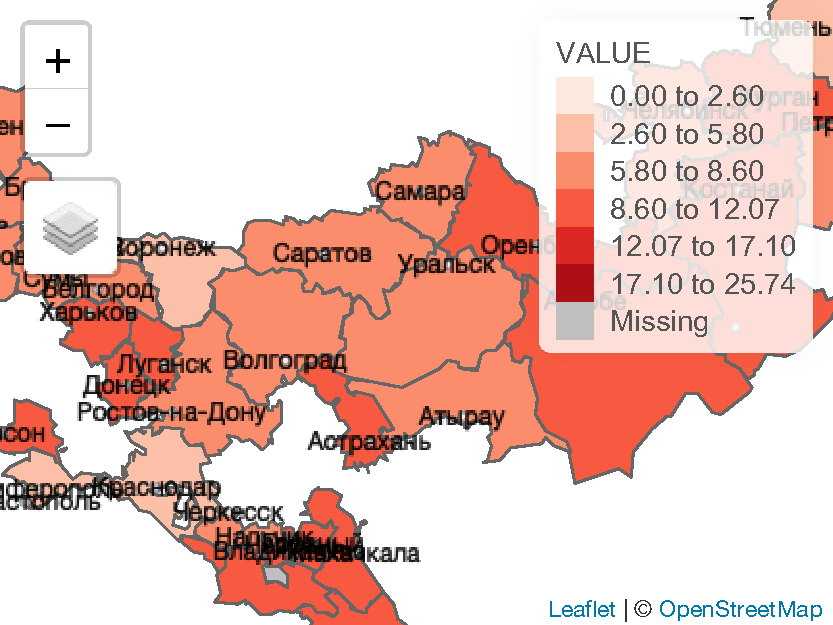
\includegraphics[width=1\linewidth]{02-Demography_files/figure-latex/unnamed-chunk-11-1}

\begin{quote}
Коэффициент миграционного прироста на 2016 г.
\end{quote}

\bibliography{articles.bib,packages.bib}


\end{document}
